\documentclass{book}
\usepackage[a4paper,top=2.5cm,bottom=2.5cm,left=2.5cm,right=2.5cm]{geometry}
\usepackage{makeidx}
\usepackage{natbib}
\usepackage{graphicx}
\usepackage{multicol}
\usepackage{float}
\usepackage{listings}
\usepackage{color}
\usepackage{ifthen}
\usepackage[table]{xcolor}
\usepackage{textcomp}
\usepackage{alltt}
\usepackage{ifpdf}
\ifpdf
\usepackage[pdftex,
            pagebackref=true,
            colorlinks=true,
            linkcolor=blue,
            unicode
           ]{hyperref}
\else
\usepackage[ps2pdf,
            pagebackref=true,
            colorlinks=true,
            linkcolor=blue,
            unicode
           ]{hyperref}
\usepackage{pspicture}
\fi
\usepackage[utf8]{inputenc}
\usepackage{mathptmx}
\usepackage[scaled=.90]{helvet}
\usepackage{courier}
\usepackage{sectsty}
\usepackage{amssymb}
\usepackage[titles]{tocloft}
\usepackage{doxygen}
\lstset{language=C++,inputencoding=utf8,basicstyle=\footnotesize,breaklines=true,breakatwhitespace=true,tabsize=4,numbers=left }
\makeindex
\setcounter{tocdepth}{3}
\renewcommand{\footrulewidth}{0.4pt}
\renewcommand{\familydefault}{\sfdefault}
\hfuzz=15pt
\setlength{\emergencystretch}{15pt}
\hbadness=750
\tolerance=750
\begin{document}
\hypersetup{pageanchor=false,citecolor=blue}
\begin{titlepage}
\vspace*{7cm}
\begin{center}
{\Large Thread\-Pool\-Timer }\\
\vspace*{1cm}
{\large Generated by Doxygen 1.8.3.1}\\
\vspace*{0.5cm}
{\small Tue Aug 13 2013 23:33:20}\\
\end{center}
\end{titlepage}
\clearemptydoublepage
\pagenumbering{roman}
\tableofcontents
\clearemptydoublepage
\pagenumbering{arabic}
\hypersetup{pageanchor=true,citecolor=blue}
\chapter{Namespace Index}
\section{Namespace List}
Here is a list of all namespaces with brief descriptions\-:\begin{DoxyCompactList}
\item\contentsline{section}{\hyperlink{namespaceThreadPoolTimer}{Thread\-Pool\-Timer} }{\pageref{namespaceThreadPoolTimer}}{}
\end{DoxyCompactList}

\chapter{Hierarchical Index}
\section{Class Hierarchy}
This inheritance list is sorted roughly, but not completely, alphabetically\-:\begin{DoxyCompactList}
\item runtime\-\_\-error\begin{DoxyCompactList}
\item \contentsline{section}{Thread\-Pool\-Timer\-:\-:Thread\-Pool\-Timer\-Exception}{\pageref{classThreadPoolTimer_1_1ThreadPoolTimerException}}{}
\begin{DoxyCompactList}
\item \contentsline{section}{Thread\-Pool\-Timer\-:\-:Timer\-Exception}{\pageref{classThreadPoolTimer_1_1TimerException}}{}
\end{DoxyCompactList}
\end{DoxyCompactList}
\item \contentsline{section}{Thread\-Pool\-Timer\-:\-:Timer}{\pageref{classThreadPoolTimer_1_1Timer}}{}
\item \contentsline{section}{Thread\-Pool\-Timer\-:\-:Timer\-Impl}{\pageref{classThreadPoolTimer_1_1TimerImpl}}{}
\item \contentsline{section}{Thread\-Pool\-Timer\-:\-:Timer\-Run\-Loop}{\pageref{classThreadPoolTimer_1_1TimerRunLoop}}{}
\end{DoxyCompactList}

\chapter{Class Index}
\section{Class List}
Here are the classes, structs, unions and interfaces with brief descriptions\-:\begin{DoxyCompactList}
\item\contentsline{section}{\hyperlink{classThreadPoolTimer_1_1ThreadPoolTimerException}{Thread\-Pool\-Timer\-::\-Thread\-Pool\-Timer\-Exception} }{\pageref{classThreadPoolTimer_1_1ThreadPoolTimerException}}{}
\item\contentsline{section}{\hyperlink{classThreadPoolTimer_1_1Timer}{Thread\-Pool\-Timer\-::\-Timer} \\*Asynchronous timer object }{\pageref{classThreadPoolTimer_1_1Timer}}{}
\item\contentsline{section}{\hyperlink{classThreadPoolTimer_1_1TimerException}{Thread\-Pool\-Timer\-::\-Timer\-Exception} }{\pageref{classThreadPoolTimer_1_1TimerException}}{}
\end{DoxyCompactList}

\chapter{File Index}
\section{File List}
Here is a list of all files with brief descriptions\-:\begin{DoxyCompactList}
\item\contentsline{section}{\hyperlink{macro_8hpp}{macro.\-hpp} }{\pageref{macro_8hpp}}{}
\item\contentsline{section}{\hyperlink{thread__pool__timer__exception_8cpp}{thread\-\_\-pool\-\_\-timer\-\_\-exception.\-cpp} }{\pageref{thread__pool__timer__exception_8cpp}}{}
\item\contentsline{section}{\hyperlink{thread__pool__timer__exception_8hpp}{thread\-\_\-pool\-\_\-timer\-\_\-exception.\-hpp} }{\pageref{thread__pool__timer__exception_8hpp}}{}
\item\contentsline{section}{\hyperlink{threadpooltimertest_8cpp}{threadpooltimertest.\-cpp} }{\pageref{threadpooltimertest_8cpp}}{}
\item\contentsline{section}{\hyperlink{timer_8cpp}{timer.\-cpp} }{\pageref{timer_8cpp}}{}
\item\contentsline{section}{\hyperlink{timer__impl_8cpp}{timer\-\_\-impl.\-cpp} }{\pageref{timer__impl_8cpp}}{}
\item\contentsline{section}{\hyperlink{timer__impl_8hpp}{timer\-\_\-impl.\-hpp} }{\pageref{timer__impl_8hpp}}{}
\item\contentsline{section}{\hyperlink{timer__run__loop_8cpp}{timer\-\_\-run\-\_\-loop.\-cpp} }{\pageref{timer__run__loop_8cpp}}{}
\item\contentsline{section}{\hyperlink{timer__run__loop_8hpp}{timer\-\_\-run\-\_\-loop.\-hpp} }{\pageref{timer__run__loop_8hpp}}{}
\item\contentsline{section}{\hyperlink{tp__timer_8hpp}{tp\-\_\-timer.\-hpp} }{\pageref{tp__timer_8hpp}}{}
\end{DoxyCompactList}

\chapter{Namespace Documentation}
\hypertarget{namespaceThreadPoolTimer}{\section{Thread\-Pool\-Timer Namespace Reference}
\label{namespaceThreadPoolTimer}\index{Thread\-Pool\-Timer@{Thread\-Pool\-Timer}}
}
\subsection*{Classes}
\begin{DoxyCompactItemize}
\item 
class \hyperlink{classThreadPoolTimer_1_1ThreadPoolTimerException}{Thread\-Pool\-Timer\-Exception}
\item 
class \hyperlink{classThreadPoolTimer_1_1TimerImpl}{Timer\-Impl}
\item 
class \hyperlink{classThreadPoolTimer_1_1TimerRunLoop}{Timer\-Run\-Loop}
\item 
class \hyperlink{classThreadPoolTimer_1_1TimerException}{Timer\-Exception}
\item 
class \hyperlink{classThreadPoolTimer_1_1Timer}{Timer}
\end{DoxyCompactItemize}
\subsection*{Functions}
\begin{DoxyCompactItemize}
\item 
bool \hyperlink{namespaceThreadPoolTimer_ab1935fa1c986ecd5a35bf71601544656}{timer\-Compare} (\hyperlink{classThreadPoolTimer_1_1TimerImpl}{Timer\-Impl} $\ast$timer\-A, \hyperlink{classThreadPoolTimer_1_1TimerImpl}{Timer\-Impl} $\ast$timer\-B)
\end{DoxyCompactItemize}


\subsection{Function Documentation}
\hypertarget{namespaceThreadPoolTimer_ab1935fa1c986ecd5a35bf71601544656}{\index{Thread\-Pool\-Timer@{Thread\-Pool\-Timer}!timer\-Compare@{timer\-Compare}}
\index{timer\-Compare@{timer\-Compare}!ThreadPoolTimer@{Thread\-Pool\-Timer}}
\subsubsection[{timer\-Compare}]{\setlength{\rightskip}{0pt plus 5cm}bool Thread\-Pool\-Timer\-::timer\-Compare (
\begin{DoxyParamCaption}
\item[{Timer\-Impl $\ast$}]{timer\-A, }
\item[{Timer\-Impl $\ast$}]{timer\-B}
\end{DoxyParamCaption}
)}}\label{namespaceThreadPoolTimer_ab1935fa1c986ecd5a35bf71601544656}

\chapter{Class Documentation}
\hypertarget{classThreadPoolTimer_1_1ThreadPoolTimerException}{\section{Thread\-Pool\-Timer\-:\-:Thread\-Pool\-Timer\-Exception Class Reference}
\label{classThreadPoolTimer_1_1ThreadPoolTimerException}\index{Thread\-Pool\-Timer\-::\-Thread\-Pool\-Timer\-Exception@{Thread\-Pool\-Timer\-::\-Thread\-Pool\-Timer\-Exception}}
}


{\ttfamily \#include $<$thread\-\_\-pool\-\_\-timer\-\_\-exception.\-hpp$>$}

Inheritance diagram for Thread\-Pool\-Timer\-:\-:Thread\-Pool\-Timer\-Exception\-:\begin{figure}[H]
\begin{center}
\leavevmode
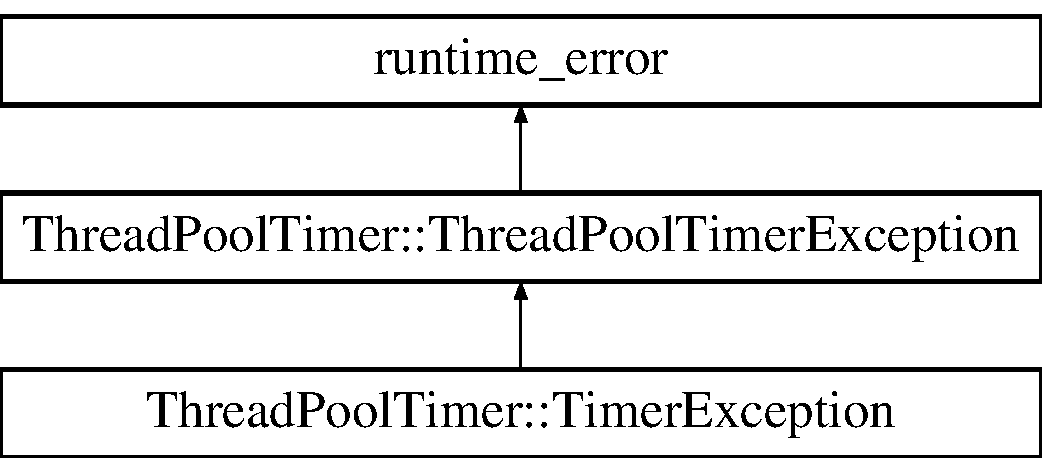
\includegraphics[height=3.000000cm]{classThreadPoolTimer_1_1ThreadPoolTimerException}
\end{center}
\end{figure}
\subsection*{Public Member Functions}
\begin{DoxyCompactItemize}
\item 
\hyperlink{classThreadPoolTimer_1_1ThreadPoolTimerException_ae8c93063905438c07aab0d52997a1959}{Thread\-Pool\-Timer\-Exception} (const char $\ast$msg)
\end{DoxyCompactItemize}


\subsection{Constructor \& Destructor Documentation}
\hypertarget{classThreadPoolTimer_1_1ThreadPoolTimerException_ae8c93063905438c07aab0d52997a1959}{\index{Thread\-Pool\-Timer\-::\-Thread\-Pool\-Timer\-Exception@{Thread\-Pool\-Timer\-::\-Thread\-Pool\-Timer\-Exception}!Thread\-Pool\-Timer\-Exception@{Thread\-Pool\-Timer\-Exception}}
\index{Thread\-Pool\-Timer\-Exception@{Thread\-Pool\-Timer\-Exception}!ThreadPoolTimer::ThreadPoolTimerException@{Thread\-Pool\-Timer\-::\-Thread\-Pool\-Timer\-Exception}}
\subsubsection[{Thread\-Pool\-Timer\-Exception}]{\setlength{\rightskip}{0pt plus 5cm}Thread\-Pool\-Timer\-::\-Thread\-Pool\-Timer\-Exception\-::\-Thread\-Pool\-Timer\-Exception (
\begin{DoxyParamCaption}
\item[{const char $\ast$}]{msg}
\end{DoxyParamCaption}
)}}\label{classThreadPoolTimer_1_1ThreadPoolTimerException_ae8c93063905438c07aab0d52997a1959}


The documentation for this class was generated from the following files\-:\begin{DoxyCompactItemize}
\item 
\hyperlink{thread__pool__timer__exception_8hpp}{thread\-\_\-pool\-\_\-timer\-\_\-exception.\-hpp}\item 
\hyperlink{thread__pool__timer__exception_8cpp}{thread\-\_\-pool\-\_\-timer\-\_\-exception.\-cpp}\end{DoxyCompactItemize}

\hypertarget{classThreadPoolTimer_1_1Timer}{\section{Thread\-Pool\-Timer\-:\-:Timer Class Reference}
\label{classThreadPoolTimer_1_1Timer}\index{Thread\-Pool\-Timer\-::\-Timer@{Thread\-Pool\-Timer\-::\-Timer}}
}


Asynchronous timer object.  




{\ttfamily \#include $<$tp\-\_\-timer.\-hpp$>$}

\subsection*{Public Member Functions}
\begin{DoxyCompactItemize}
\item 
\hyperlink{classThreadPoolTimer_1_1Timer_a931fa92e610af4ac53f665471b5516b4}{Timer} (std\-::function$<$ void()$>$ callback, const std\-::chrono\-::nanoseconds \&interval=std\-::chrono\-::nanoseconds(0))
\begin{DoxyCompactList}\small\item\em Construct a \hyperlink{classThreadPoolTimer_1_1Timer}{Timer} object with a callback. \end{DoxyCompactList}\item 
void \hyperlink{classThreadPoolTimer_1_1Timer_a9112e65788529e3230b22dcace7421f7}{set\-Interval} (const std\-::chrono\-::nanoseconds \&interval)
\begin{DoxyCompactList}\small\item\em Set the timer's event interval. \end{DoxyCompactList}\item 
void \hyperlink{classThreadPoolTimer_1_1Timer_aed13ba283b0cd1e83697bc0d553b37d9}{set\-Enabled} (bool enabled)
\begin{DoxyCompactList}\small\item\em Enable or disable the timer. \end{DoxyCompactList}\item 
\hypertarget{classThreadPoolTimer_1_1Timer_ab2543b0d593e885335786d5b2ed81302}{bool \hyperlink{classThreadPoolTimer_1_1Timer_ab2543b0d593e885335786d5b2ed81302}{get\-Enabled} ()}\label{classThreadPoolTimer_1_1Timer_ab2543b0d593e885335786d5b2ed81302}

\begin{DoxyCompactList}\small\item\em Get the timer's enabled status. \end{DoxyCompactList}\end{DoxyCompactItemize}
\subsection*{Static Public Member Functions}
\begin{DoxyCompactItemize}
\item 
static void \hyperlink{classThreadPoolTimer_1_1Timer_afc1617ff337812f126f04ee425f48caa}{stop\-Run\-Loop} ()
\begin{DoxyCompactList}\small\item\em Stop the thread pool's run loop. \end{DoxyCompactList}\item 
static void \hyperlink{classThreadPoolTimer_1_1Timer_a5918ac320ad2bddfdbf72b0380392107}{start\-Run\-Loop} ()
\begin{DoxyCompactList}\small\item\em Start the thread pool's run loop. \end{DoxyCompactList}\end{DoxyCompactItemize}


\subsection{Detailed Description}
Asynchronous timer object. 

\subsection{Constructor \& Destructor Documentation}
\hypertarget{classThreadPoolTimer_1_1Timer_a931fa92e610af4ac53f665471b5516b4}{\index{Thread\-Pool\-Timer\-::\-Timer@{Thread\-Pool\-Timer\-::\-Timer}!Timer@{Timer}}
\index{Timer@{Timer}!ThreadPoolTimer::Timer@{Thread\-Pool\-Timer\-::\-Timer}}
\subsubsection[{Timer}]{\setlength{\rightskip}{0pt plus 5cm}Thread\-Pool\-Timer\-::\-Timer\-::\-Timer (
\begin{DoxyParamCaption}
\item[{std\-::function$<$ void()$>$}]{callback, }
\item[{const std\-::chrono\-::nanoseconds \&}]{interval = {\ttfamily std\-:\-:chrono\-:\-:nanoseconds(0)}}
\end{DoxyParamCaption}
)}}\label{classThreadPoolTimer_1_1Timer_a931fa92e610af4ac53f665471b5516b4}


Construct a \hyperlink{classThreadPoolTimer_1_1Timer}{Timer} object with a callback. 


\begin{DoxyParams}{Parameters}
{\em callback} & Any callable target (lambda expressions, bind expressions, etc) \\
\hline
{\em interval} & See \hyperlink{classThreadPoolTimer_1_1Timer_a9112e65788529e3230b22dcace7421f7}{set\-Interval( const std\-::chrono\-::nanoseconds \&interval )}; \\
\hline
\end{DoxyParams}


\subsection{Member Function Documentation}
\hypertarget{classThreadPoolTimer_1_1Timer_aed13ba283b0cd1e83697bc0d553b37d9}{\index{Thread\-Pool\-Timer\-::\-Timer@{Thread\-Pool\-Timer\-::\-Timer}!set\-Enabled@{set\-Enabled}}
\index{set\-Enabled@{set\-Enabled}!ThreadPoolTimer::Timer@{Thread\-Pool\-Timer\-::\-Timer}}
\subsubsection[{set\-Enabled}]{\setlength{\rightskip}{0pt plus 5cm}void Thread\-Pool\-Timer\-::\-Timer\-::set\-Enabled (
\begin{DoxyParamCaption}
\item[{bool}]{enabled}
\end{DoxyParamCaption}
)}}\label{classThreadPoolTimer_1_1Timer_aed13ba283b0cd1e83697bc0d553b37d9}


Enable or disable the timer. 

Enabling the timer registers the timer with the thread pool, and events will begin to trigger at the specified interval. Attempting to enable the timer without previously setting an interval, or while the interval is set to zero, will throw a \hyperlink{classThreadPoolTimer_1_1TimerException}{Timer\-Exception}. Disabling the timer de-\/registers it from the thread pool. No further events will fire after \hyperlink{classThreadPoolTimer_1_1Timer_aed13ba283b0cd1e83697bc0d553b37d9}{set\-Enabled()} returns. It is possible, however, that an event may fire after \hyperlink{classThreadPoolTimer_1_1Timer_aed13ba283b0cd1e83697bc0d553b37d9}{set\-Enabled()} is called, but before it returns. 
\begin{DoxyParams}{Parameters}
{\em enabled} & true to enable the timer; false to disable \\
\hline
\end{DoxyParams}
\hypertarget{classThreadPoolTimer_1_1Timer_a9112e65788529e3230b22dcace7421f7}{\index{Thread\-Pool\-Timer\-::\-Timer@{Thread\-Pool\-Timer\-::\-Timer}!set\-Interval@{set\-Interval}}
\index{set\-Interval@{set\-Interval}!ThreadPoolTimer::Timer@{Thread\-Pool\-Timer\-::\-Timer}}
\subsubsection[{set\-Interval}]{\setlength{\rightskip}{0pt plus 5cm}void Thread\-Pool\-Timer\-::\-Timer\-::set\-Interval (
\begin{DoxyParamCaption}
\item[{const std\-::chrono\-::nanoseconds \&}]{interval}
\end{DoxyParamCaption}
)}}\label{classThreadPoolTimer_1_1Timer_a9112e65788529e3230b22dcace7421f7}


Set the timer's event interval. 


\begin{DoxyParams}{Parameters}
{\em interval} & The timing interval specified in nanoseconds. Any std\-::chrono\-::duration value can be converted to nanoseconds with std\-::chrono\-::duration\-\_\-cast$<$std\-::chrono\-::nanoseconds(x). If the timer is enabled when the interval is set, the timer will first be disabled, the interval set, and then re-\/enabled. Setting the interval to 0 will disable the timer. \\
\hline
\end{DoxyParams}
\hypertarget{classThreadPoolTimer_1_1Timer_a5918ac320ad2bddfdbf72b0380392107}{\index{Thread\-Pool\-Timer\-::\-Timer@{Thread\-Pool\-Timer\-::\-Timer}!start\-Run\-Loop@{start\-Run\-Loop}}
\index{start\-Run\-Loop@{start\-Run\-Loop}!ThreadPoolTimer::Timer@{Thread\-Pool\-Timer\-::\-Timer}}
\subsubsection[{start\-Run\-Loop}]{\setlength{\rightskip}{0pt plus 5cm}void Thread\-Pool\-Timer\-::\-Timer\-::start\-Run\-Loop (
\begin{DoxyParamCaption}
{}
\end{DoxyParamCaption}
)\hspace{0.3cm}{\ttfamily [static]}}}\label{classThreadPoolTimer_1_1Timer_a5918ac320ad2bddfdbf72b0380392107}


Start the thread pool's run loop. 

This should only be called if the run loop has previously been stopped with \hyperlink{classThreadPoolTimer_1_1Timer_afc1617ff337812f126f04ee425f48caa}{stop\-Run\-Loop()}. The run loop is normally started automatically when the first \hyperlink{classThreadPoolTimer_1_1Timer}{Timer} object is enabled. \hypertarget{classThreadPoolTimer_1_1Timer_afc1617ff337812f126f04ee425f48caa}{\index{Thread\-Pool\-Timer\-::\-Timer@{Thread\-Pool\-Timer\-::\-Timer}!stop\-Run\-Loop@{stop\-Run\-Loop}}
\index{stop\-Run\-Loop@{stop\-Run\-Loop}!ThreadPoolTimer::Timer@{Thread\-Pool\-Timer\-::\-Timer}}
\subsubsection[{stop\-Run\-Loop}]{\setlength{\rightskip}{0pt plus 5cm}void Thread\-Pool\-Timer\-::\-Timer\-::stop\-Run\-Loop (
\begin{DoxyParamCaption}
{}
\end{DoxyParamCaption}
)\hspace{0.3cm}{\ttfamily [static]}}}\label{classThreadPoolTimer_1_1Timer_afc1617ff337812f126f04ee425f48caa}


Stop the thread pool's run loop. 

After the thread pool's run loop is stopped, no further events will trigger on any registered \hyperlink{classThreadPoolTimer_1_1Timer}{Timer} objects. 

The documentation for this class was generated from the following files\-:\begin{DoxyCompactItemize}
\item 
tp\-\_\-timer.\-hpp\item 
timer.\-cpp\end{DoxyCompactItemize}

\hypertarget{classThreadPoolTimer_1_1TimerException}{\section{Thread\-Pool\-Timer\-:\-:Timer\-Exception Class Reference}
\label{classThreadPoolTimer_1_1TimerException}\index{Thread\-Pool\-Timer\-::\-Timer\-Exception@{Thread\-Pool\-Timer\-::\-Timer\-Exception}}
}
Inheritance diagram for Thread\-Pool\-Timer\-:\-:Timer\-Exception\-:\begin{figure}[H]
\begin{center}
\leavevmode
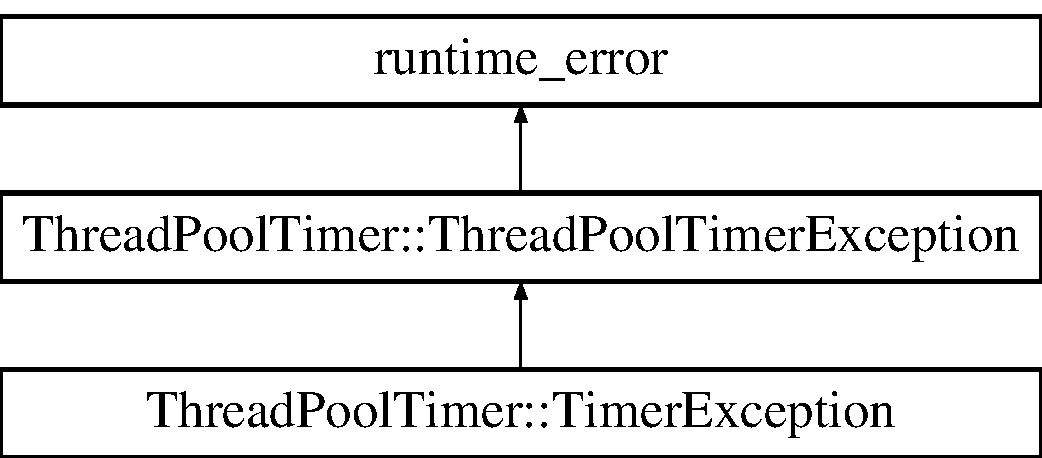
\includegraphics[height=3.000000cm]{classThreadPoolTimer_1_1TimerException}
\end{center}
\end{figure}
\subsection*{Public Member Functions}
\begin{DoxyCompactItemize}
\item 
\hypertarget{classThreadPoolTimer_1_1TimerException_aa64e837274d9cc224de2bbe0d5e9a3b9}{{\bfseries Timer\-Exception} (const char $\ast$msg)}\label{classThreadPoolTimer_1_1TimerException_aa64e837274d9cc224de2bbe0d5e9a3b9}

\end{DoxyCompactItemize}


The documentation for this class was generated from the following file\-:\begin{DoxyCompactItemize}
\item 
tp\-\_\-timer.\-hpp\end{DoxyCompactItemize}

\hypertarget{classThreadPoolTimer_1_1TimerImpl}{\section{Thread\-Pool\-Timer\-:\-:Timer\-Impl Class Reference}
\label{classThreadPoolTimer_1_1TimerImpl}\index{Thread\-Pool\-Timer\-::\-Timer\-Impl@{Thread\-Pool\-Timer\-::\-Timer\-Impl}}
}


{\ttfamily \#include $<$timer\-\_\-impl.\-hpp$>$}

\subsection*{Public Member Functions}
\begin{DoxyCompactItemize}
\item 
\hyperlink{classThreadPoolTimer_1_1TimerImpl_adbb7de16348e9819dabc9319e4dfd4d0}{Timer\-Impl} (std\-::function$<$ void()$>$ task)
\item 
\hyperlink{classThreadPoolTimer_1_1TimerImpl_a97e1cf4b5bc2dd00c723b646384cd496}{$\sim$\-Timer\-Impl} ()
\item 
void \hyperlink{classThreadPoolTimer_1_1TimerImpl_a50873e7385216f0adb1e188281e25d93}{set\-Interval} (const std\-::chrono\-::nanoseconds \&interval)
\item 
const std\-::chrono\-::nanoseconds \& \hyperlink{classThreadPoolTimer_1_1TimerImpl_a5d2786dbaa14891acd5330b61c1a4bda}{get\-Interval} ()
\item 
void \hyperlink{classThreadPoolTimer_1_1TimerImpl_ab1be2145856231b15f1abc156ee1c508}{set\-Enabled} (bool enabled)
\item 
bool \hyperlink{classThreadPoolTimer_1_1TimerImpl_a588fd97294a1eb941670b49d6829947e}{get\-Enabled} ()
\item 
void \hyperlink{classThreadPoolTimer_1_1TimerImpl_a82e3056f281fe397ee7e297a573f97f6}{set\-Next\-Trigger} (const std\-::chrono\-::steady\-\_\-clock\-::time\-\_\-point \&\hyperlink{classThreadPoolTimer_1_1TimerImpl_ac89984aaaad00020982dc23205672aa5}{trigger})
\item 
std\-::chrono\-::steady\-\_\-clock\-::time\-\_\-point \& \hyperlink{classThreadPoolTimer_1_1TimerImpl_ad3a5a4a2fabfd54b069f5f30c65f2fea}{get\-Next\-Trigger} ()
\item 
void \hyperlink{classThreadPoolTimer_1_1TimerImpl_ac89984aaaad00020982dc23205672aa5}{trigger} ()
\end{DoxyCompactItemize}
\subsection*{Static Public Member Functions}
\begin{DoxyCompactItemize}
\item 
static void \hyperlink{classThreadPoolTimer_1_1TimerImpl_afc1e2e4b54e377e665fa04c6273e599d}{stop\-Run\-Loop} ()
\item 
static void \hyperlink{classThreadPoolTimer_1_1TimerImpl_a593b3028fedb0b0d135313148232f3cc}{start\-Run\-Loop} ()
\end{DoxyCompactItemize}


\subsection{Constructor \& Destructor Documentation}
\hypertarget{classThreadPoolTimer_1_1TimerImpl_adbb7de16348e9819dabc9319e4dfd4d0}{\index{Thread\-Pool\-Timer\-::\-Timer\-Impl@{Thread\-Pool\-Timer\-::\-Timer\-Impl}!Timer\-Impl@{Timer\-Impl}}
\index{Timer\-Impl@{Timer\-Impl}!ThreadPoolTimer::TimerImpl@{Thread\-Pool\-Timer\-::\-Timer\-Impl}}
\subsubsection[{Timer\-Impl}]{\setlength{\rightskip}{0pt plus 5cm}Thread\-Pool\-Timer\-::\-Timer\-Impl\-::\-Timer\-Impl (
\begin{DoxyParamCaption}
\item[{std\-::function$<$ void()$>$}]{task}
\end{DoxyParamCaption}
)}}\label{classThreadPoolTimer_1_1TimerImpl_adbb7de16348e9819dabc9319e4dfd4d0}
\hypertarget{classThreadPoolTimer_1_1TimerImpl_a97e1cf4b5bc2dd00c723b646384cd496}{\index{Thread\-Pool\-Timer\-::\-Timer\-Impl@{Thread\-Pool\-Timer\-::\-Timer\-Impl}!$\sim$\-Timer\-Impl@{$\sim$\-Timer\-Impl}}
\index{$\sim$\-Timer\-Impl@{$\sim$\-Timer\-Impl}!ThreadPoolTimer::TimerImpl@{Thread\-Pool\-Timer\-::\-Timer\-Impl}}
\subsubsection[{$\sim$\-Timer\-Impl}]{\setlength{\rightskip}{0pt plus 5cm}Thread\-Pool\-Timer\-::\-Timer\-Impl\-::$\sim$\-Timer\-Impl (
\begin{DoxyParamCaption}
{}
\end{DoxyParamCaption}
)}}\label{classThreadPoolTimer_1_1TimerImpl_a97e1cf4b5bc2dd00c723b646384cd496}


\subsection{Member Function Documentation}
\hypertarget{classThreadPoolTimer_1_1TimerImpl_a588fd97294a1eb941670b49d6829947e}{\index{Thread\-Pool\-Timer\-::\-Timer\-Impl@{Thread\-Pool\-Timer\-::\-Timer\-Impl}!get\-Enabled@{get\-Enabled}}
\index{get\-Enabled@{get\-Enabled}!ThreadPoolTimer::TimerImpl@{Thread\-Pool\-Timer\-::\-Timer\-Impl}}
\subsubsection[{get\-Enabled}]{\setlength{\rightskip}{0pt plus 5cm}bool Thread\-Pool\-Timer\-::\-Timer\-Impl\-::get\-Enabled (
\begin{DoxyParamCaption}
{}
\end{DoxyParamCaption}
)}}\label{classThreadPoolTimer_1_1TimerImpl_a588fd97294a1eb941670b49d6829947e}
\hypertarget{classThreadPoolTimer_1_1TimerImpl_a5d2786dbaa14891acd5330b61c1a4bda}{\index{Thread\-Pool\-Timer\-::\-Timer\-Impl@{Thread\-Pool\-Timer\-::\-Timer\-Impl}!get\-Interval@{get\-Interval}}
\index{get\-Interval@{get\-Interval}!ThreadPoolTimer::TimerImpl@{Thread\-Pool\-Timer\-::\-Timer\-Impl}}
\subsubsection[{get\-Interval}]{\setlength{\rightskip}{0pt plus 5cm}const std\-::chrono\-::nanoseconds \& Thread\-Pool\-Timer\-::\-Timer\-Impl\-::get\-Interval (
\begin{DoxyParamCaption}
{}
\end{DoxyParamCaption}
)}}\label{classThreadPoolTimer_1_1TimerImpl_a5d2786dbaa14891acd5330b61c1a4bda}
\hypertarget{classThreadPoolTimer_1_1TimerImpl_ad3a5a4a2fabfd54b069f5f30c65f2fea}{\index{Thread\-Pool\-Timer\-::\-Timer\-Impl@{Thread\-Pool\-Timer\-::\-Timer\-Impl}!get\-Next\-Trigger@{get\-Next\-Trigger}}
\index{get\-Next\-Trigger@{get\-Next\-Trigger}!ThreadPoolTimer::TimerImpl@{Thread\-Pool\-Timer\-::\-Timer\-Impl}}
\subsubsection[{get\-Next\-Trigger}]{\setlength{\rightskip}{0pt plus 5cm}std\-::chrono\-::steady\-\_\-clock\-::time\-\_\-point \& Thread\-Pool\-Timer\-::\-Timer\-Impl\-::get\-Next\-Trigger (
\begin{DoxyParamCaption}
{}
\end{DoxyParamCaption}
)}}\label{classThreadPoolTimer_1_1TimerImpl_ad3a5a4a2fabfd54b069f5f30c65f2fea}
\hypertarget{classThreadPoolTimer_1_1TimerImpl_ab1be2145856231b15f1abc156ee1c508}{\index{Thread\-Pool\-Timer\-::\-Timer\-Impl@{Thread\-Pool\-Timer\-::\-Timer\-Impl}!set\-Enabled@{set\-Enabled}}
\index{set\-Enabled@{set\-Enabled}!ThreadPoolTimer::TimerImpl@{Thread\-Pool\-Timer\-::\-Timer\-Impl}}
\subsubsection[{set\-Enabled}]{\setlength{\rightskip}{0pt plus 5cm}void Thread\-Pool\-Timer\-::\-Timer\-Impl\-::set\-Enabled (
\begin{DoxyParamCaption}
\item[{bool}]{enabled}
\end{DoxyParamCaption}
)}}\label{classThreadPoolTimer_1_1TimerImpl_ab1be2145856231b15f1abc156ee1c508}
\hypertarget{classThreadPoolTimer_1_1TimerImpl_a50873e7385216f0adb1e188281e25d93}{\index{Thread\-Pool\-Timer\-::\-Timer\-Impl@{Thread\-Pool\-Timer\-::\-Timer\-Impl}!set\-Interval@{set\-Interval}}
\index{set\-Interval@{set\-Interval}!ThreadPoolTimer::TimerImpl@{Thread\-Pool\-Timer\-::\-Timer\-Impl}}
\subsubsection[{set\-Interval}]{\setlength{\rightskip}{0pt plus 5cm}void Thread\-Pool\-Timer\-::\-Timer\-Impl\-::set\-Interval (
\begin{DoxyParamCaption}
\item[{const std\-::chrono\-::nanoseconds \&}]{interval}
\end{DoxyParamCaption}
)}}\label{classThreadPoolTimer_1_1TimerImpl_a50873e7385216f0adb1e188281e25d93}
\hypertarget{classThreadPoolTimer_1_1TimerImpl_a82e3056f281fe397ee7e297a573f97f6}{\index{Thread\-Pool\-Timer\-::\-Timer\-Impl@{Thread\-Pool\-Timer\-::\-Timer\-Impl}!set\-Next\-Trigger@{set\-Next\-Trigger}}
\index{set\-Next\-Trigger@{set\-Next\-Trigger}!ThreadPoolTimer::TimerImpl@{Thread\-Pool\-Timer\-::\-Timer\-Impl}}
\subsubsection[{set\-Next\-Trigger}]{\setlength{\rightskip}{0pt plus 5cm}void Thread\-Pool\-Timer\-::\-Timer\-Impl\-::set\-Next\-Trigger (
\begin{DoxyParamCaption}
\item[{const std\-::chrono\-::steady\-\_\-clock\-::time\-\_\-point \&}]{trigger}
\end{DoxyParamCaption}
)}}\label{classThreadPoolTimer_1_1TimerImpl_a82e3056f281fe397ee7e297a573f97f6}
\hypertarget{classThreadPoolTimer_1_1TimerImpl_a593b3028fedb0b0d135313148232f3cc}{\index{Thread\-Pool\-Timer\-::\-Timer\-Impl@{Thread\-Pool\-Timer\-::\-Timer\-Impl}!start\-Run\-Loop@{start\-Run\-Loop}}
\index{start\-Run\-Loop@{start\-Run\-Loop}!ThreadPoolTimer::TimerImpl@{Thread\-Pool\-Timer\-::\-Timer\-Impl}}
\subsubsection[{start\-Run\-Loop}]{\setlength{\rightskip}{0pt plus 5cm}void Thread\-Pool\-Timer\-::\-Timer\-Impl\-::start\-Run\-Loop (
\begin{DoxyParamCaption}
{}
\end{DoxyParamCaption}
)\hspace{0.3cm}{\ttfamily [static]}}}\label{classThreadPoolTimer_1_1TimerImpl_a593b3028fedb0b0d135313148232f3cc}
\hypertarget{classThreadPoolTimer_1_1TimerImpl_afc1e2e4b54e377e665fa04c6273e599d}{\index{Thread\-Pool\-Timer\-::\-Timer\-Impl@{Thread\-Pool\-Timer\-::\-Timer\-Impl}!stop\-Run\-Loop@{stop\-Run\-Loop}}
\index{stop\-Run\-Loop@{stop\-Run\-Loop}!ThreadPoolTimer::TimerImpl@{Thread\-Pool\-Timer\-::\-Timer\-Impl}}
\subsubsection[{stop\-Run\-Loop}]{\setlength{\rightskip}{0pt plus 5cm}void Thread\-Pool\-Timer\-::\-Timer\-Impl\-::stop\-Run\-Loop (
\begin{DoxyParamCaption}
{}
\end{DoxyParamCaption}
)\hspace{0.3cm}{\ttfamily [static]}}}\label{classThreadPoolTimer_1_1TimerImpl_afc1e2e4b54e377e665fa04c6273e599d}
\hypertarget{classThreadPoolTimer_1_1TimerImpl_ac89984aaaad00020982dc23205672aa5}{\index{Thread\-Pool\-Timer\-::\-Timer\-Impl@{Thread\-Pool\-Timer\-::\-Timer\-Impl}!trigger@{trigger}}
\index{trigger@{trigger}!ThreadPoolTimer::TimerImpl@{Thread\-Pool\-Timer\-::\-Timer\-Impl}}
\subsubsection[{trigger}]{\setlength{\rightskip}{0pt plus 5cm}void Thread\-Pool\-Timer\-::\-Timer\-Impl\-::trigger (
\begin{DoxyParamCaption}
{}
\end{DoxyParamCaption}
)}}\label{classThreadPoolTimer_1_1TimerImpl_ac89984aaaad00020982dc23205672aa5}


The documentation for this class was generated from the following files\-:\begin{DoxyCompactItemize}
\item 
\hyperlink{timer__impl_8hpp}{timer\-\_\-impl.\-hpp}\item 
\hyperlink{timer__impl_8cpp}{timer\-\_\-impl.\-cpp}\end{DoxyCompactItemize}

\hypertarget{classThreadPoolTimer_1_1TimerRunLoop}{\section{Thread\-Pool\-Timer\-:\-:Timer\-Run\-Loop Class Reference}
\label{classThreadPoolTimer_1_1TimerRunLoop}\index{Thread\-Pool\-Timer\-::\-Timer\-Run\-Loop@{Thread\-Pool\-Timer\-::\-Timer\-Run\-Loop}}
}


{\ttfamily \#include $<$timer\-\_\-run\-\_\-loop.\-hpp$>$}

\subsection*{Public Member Functions}
\begin{DoxyCompactItemize}
\item 
\hyperlink{classThreadPoolTimer_1_1TimerRunLoop_a2c148c9d8d43304c9f5ce73cb3b8a929}{Timer\-Run\-Loop} ()
\item 
\hyperlink{classThreadPoolTimer_1_1TimerRunLoop_abbe4f1e81556ffef1d665b505f9a6593}{$\sim$\-Timer\-Run\-Loop} ()
\item 
bool \hyperlink{classThreadPoolTimer_1_1TimerRunLoop_a3010542f1e7d6b191223365e052d50ab}{get\-Running} ()
\item 
void \hyperlink{classThreadPoolTimer_1_1TimerRunLoop_ad021a08b2dd037f90f2228e2b22544db}{stop} ()
\item 
void \hyperlink{classThreadPoolTimer_1_1TimerRunLoop_ae94976ed95afb92b0b47b56e11cb78c7}{start} ()
\item 
void \hyperlink{classThreadPoolTimer_1_1TimerRunLoop_a84fe2cd1cbfed86d3f6c2b4dc9f785c3}{register\-Timer} (\hyperlink{classThreadPoolTimer_1_1TimerImpl}{Timer\-Impl} \&timer)
\item 
void \hyperlink{classThreadPoolTimer_1_1TimerRunLoop_a35978d0ef8e0d91808ebfa09da5c24f2}{un\-Register\-Timer} (\hyperlink{classThreadPoolTimer_1_1TimerImpl}{Timer\-Impl} \&timer)
\end{DoxyCompactItemize}
\subsection*{Static Public Member Functions}
\begin{DoxyCompactItemize}
\item 
static \hyperlink{classThreadPoolTimer_1_1TimerRunLoop}{Timer\-Run\-Loop} \& \hyperlink{classThreadPoolTimer_1_1TimerRunLoop_ad8f4868fb5c754e59a9f4ce150625c5a}{get\-Singleton} ()
\end{DoxyCompactItemize}


\subsection{Constructor \& Destructor Documentation}
\hypertarget{classThreadPoolTimer_1_1TimerRunLoop_a2c148c9d8d43304c9f5ce73cb3b8a929}{\index{Thread\-Pool\-Timer\-::\-Timer\-Run\-Loop@{Thread\-Pool\-Timer\-::\-Timer\-Run\-Loop}!Timer\-Run\-Loop@{Timer\-Run\-Loop}}
\index{Timer\-Run\-Loop@{Timer\-Run\-Loop}!ThreadPoolTimer::TimerRunLoop@{Thread\-Pool\-Timer\-::\-Timer\-Run\-Loop}}
\subsubsection[{Timer\-Run\-Loop}]{\setlength{\rightskip}{0pt plus 5cm}Thread\-Pool\-Timer\-::\-Timer\-Run\-Loop\-::\-Timer\-Run\-Loop (
\begin{DoxyParamCaption}
{}
\end{DoxyParamCaption}
)}}\label{classThreadPoolTimer_1_1TimerRunLoop_a2c148c9d8d43304c9f5ce73cb3b8a929}
\hypertarget{classThreadPoolTimer_1_1TimerRunLoop_abbe4f1e81556ffef1d665b505f9a6593}{\index{Thread\-Pool\-Timer\-::\-Timer\-Run\-Loop@{Thread\-Pool\-Timer\-::\-Timer\-Run\-Loop}!$\sim$\-Timer\-Run\-Loop@{$\sim$\-Timer\-Run\-Loop}}
\index{$\sim$\-Timer\-Run\-Loop@{$\sim$\-Timer\-Run\-Loop}!ThreadPoolTimer::TimerRunLoop@{Thread\-Pool\-Timer\-::\-Timer\-Run\-Loop}}
\subsubsection[{$\sim$\-Timer\-Run\-Loop}]{\setlength{\rightskip}{0pt plus 5cm}Thread\-Pool\-Timer\-::\-Timer\-Run\-Loop\-::$\sim$\-Timer\-Run\-Loop (
\begin{DoxyParamCaption}
{}
\end{DoxyParamCaption}
)}}\label{classThreadPoolTimer_1_1TimerRunLoop_abbe4f1e81556ffef1d665b505f9a6593}


\subsection{Member Function Documentation}
\hypertarget{classThreadPoolTimer_1_1TimerRunLoop_a3010542f1e7d6b191223365e052d50ab}{\index{Thread\-Pool\-Timer\-::\-Timer\-Run\-Loop@{Thread\-Pool\-Timer\-::\-Timer\-Run\-Loop}!get\-Running@{get\-Running}}
\index{get\-Running@{get\-Running}!ThreadPoolTimer::TimerRunLoop@{Thread\-Pool\-Timer\-::\-Timer\-Run\-Loop}}
\subsubsection[{get\-Running}]{\setlength{\rightskip}{0pt plus 5cm}bool Thread\-Pool\-Timer\-::\-Timer\-Run\-Loop\-::get\-Running (
\begin{DoxyParamCaption}
{}
\end{DoxyParamCaption}
)}}\label{classThreadPoolTimer_1_1TimerRunLoop_a3010542f1e7d6b191223365e052d50ab}
\hypertarget{classThreadPoolTimer_1_1TimerRunLoop_ad8f4868fb5c754e59a9f4ce150625c5a}{\index{Thread\-Pool\-Timer\-::\-Timer\-Run\-Loop@{Thread\-Pool\-Timer\-::\-Timer\-Run\-Loop}!get\-Singleton@{get\-Singleton}}
\index{get\-Singleton@{get\-Singleton}!ThreadPoolTimer::TimerRunLoop@{Thread\-Pool\-Timer\-::\-Timer\-Run\-Loop}}
\subsubsection[{get\-Singleton}]{\setlength{\rightskip}{0pt plus 5cm}{\bf Timer\-Run\-Loop} \& Thread\-Pool\-Timer\-::\-Timer\-Run\-Loop\-::get\-Singleton (
\begin{DoxyParamCaption}
{}
\end{DoxyParamCaption}
)\hspace{0.3cm}{\ttfamily [static]}}}\label{classThreadPoolTimer_1_1TimerRunLoop_ad8f4868fb5c754e59a9f4ce150625c5a}
\hypertarget{classThreadPoolTimer_1_1TimerRunLoop_a84fe2cd1cbfed86d3f6c2b4dc9f785c3}{\index{Thread\-Pool\-Timer\-::\-Timer\-Run\-Loop@{Thread\-Pool\-Timer\-::\-Timer\-Run\-Loop}!register\-Timer@{register\-Timer}}
\index{register\-Timer@{register\-Timer}!ThreadPoolTimer::TimerRunLoop@{Thread\-Pool\-Timer\-::\-Timer\-Run\-Loop}}
\subsubsection[{register\-Timer}]{\setlength{\rightskip}{0pt plus 5cm}void Thread\-Pool\-Timer\-::\-Timer\-Run\-Loop\-::register\-Timer (
\begin{DoxyParamCaption}
\item[{{\bf Timer\-Impl} \&}]{timer}
\end{DoxyParamCaption}
)}}\label{classThreadPoolTimer_1_1TimerRunLoop_a84fe2cd1cbfed86d3f6c2b4dc9f785c3}
\hypertarget{classThreadPoolTimer_1_1TimerRunLoop_ae94976ed95afb92b0b47b56e11cb78c7}{\index{Thread\-Pool\-Timer\-::\-Timer\-Run\-Loop@{Thread\-Pool\-Timer\-::\-Timer\-Run\-Loop}!start@{start}}
\index{start@{start}!ThreadPoolTimer::TimerRunLoop@{Thread\-Pool\-Timer\-::\-Timer\-Run\-Loop}}
\subsubsection[{start}]{\setlength{\rightskip}{0pt plus 5cm}void Thread\-Pool\-Timer\-::\-Timer\-Run\-Loop\-::start (
\begin{DoxyParamCaption}
{}
\end{DoxyParamCaption}
)}}\label{classThreadPoolTimer_1_1TimerRunLoop_ae94976ed95afb92b0b47b56e11cb78c7}
\hypertarget{classThreadPoolTimer_1_1TimerRunLoop_ad021a08b2dd037f90f2228e2b22544db}{\index{Thread\-Pool\-Timer\-::\-Timer\-Run\-Loop@{Thread\-Pool\-Timer\-::\-Timer\-Run\-Loop}!stop@{stop}}
\index{stop@{stop}!ThreadPoolTimer::TimerRunLoop@{Thread\-Pool\-Timer\-::\-Timer\-Run\-Loop}}
\subsubsection[{stop}]{\setlength{\rightskip}{0pt plus 5cm}void Thread\-Pool\-Timer\-::\-Timer\-Run\-Loop\-::stop (
\begin{DoxyParamCaption}
{}
\end{DoxyParamCaption}
)}}\label{classThreadPoolTimer_1_1TimerRunLoop_ad021a08b2dd037f90f2228e2b22544db}
\hypertarget{classThreadPoolTimer_1_1TimerRunLoop_a35978d0ef8e0d91808ebfa09da5c24f2}{\index{Thread\-Pool\-Timer\-::\-Timer\-Run\-Loop@{Thread\-Pool\-Timer\-::\-Timer\-Run\-Loop}!un\-Register\-Timer@{un\-Register\-Timer}}
\index{un\-Register\-Timer@{un\-Register\-Timer}!ThreadPoolTimer::TimerRunLoop@{Thread\-Pool\-Timer\-::\-Timer\-Run\-Loop}}
\subsubsection[{un\-Register\-Timer}]{\setlength{\rightskip}{0pt plus 5cm}void Thread\-Pool\-Timer\-::\-Timer\-Run\-Loop\-::un\-Register\-Timer (
\begin{DoxyParamCaption}
\item[{{\bf Timer\-Impl} \&}]{timer}
\end{DoxyParamCaption}
)}}\label{classThreadPoolTimer_1_1TimerRunLoop_a35978d0ef8e0d91808ebfa09da5c24f2}


The documentation for this class was generated from the following files\-:\begin{DoxyCompactItemize}
\item 
\hyperlink{timer__run__loop_8hpp}{timer\-\_\-run\-\_\-loop.\-hpp}\item 
\hyperlink{timer__run__loop_8cpp}{timer\-\_\-run\-\_\-loop.\-cpp}\end{DoxyCompactItemize}

\chapter{File Documentation}
\hypertarget{macro_8hpp}{\section{macro.\-hpp File Reference}
\label{macro_8hpp}\index{macro.\-hpp@{macro.\-hpp}}
}
{\ttfamily \#include $<$cstdlib$>$}\\*
{\ttfamily \#include $<$string$>$}\\*
{\ttfamily \#include \char`\"{}thread\-\_\-pool\-\_\-timer\-\_\-exception.\-hpp\char`\"{}}\\*
\subsection*{Macros}
\begin{DoxyCompactItemize}
\item 
\#define \hyperlink{macro_8hpp_af8df3547bfde53a5acb93e2607b0034a}{D\-I\-S\-A\-L\-L\-O\-W\-\_\-\-C\-O\-P\-Y\-\_\-\-A\-N\-D\-\_\-\-A\-S\-S\-I\-G\-N}(Type\-Name)
\item 
\#define \hyperlink{macro_8hpp_ac14433ff87451a3fdd20a0ab3ef7e42c}{R\-U\-N\-T\-I\-M\-E\-\_\-\-E\-X\-C\-E\-P\-T\-I\-O\-N\-\_\-\-S\-U\-B\-C\-L\-A\-S\-S}(Class\-Name, Super\-Class\-Name)
\end{DoxyCompactItemize}


\subsection{Macro Definition Documentation}
\hypertarget{macro_8hpp_af8df3547bfde53a5acb93e2607b0034a}{\index{macro.\-hpp@{macro.\-hpp}!D\-I\-S\-A\-L\-L\-O\-W\-\_\-\-C\-O\-P\-Y\-\_\-\-A\-N\-D\-\_\-\-A\-S\-S\-I\-G\-N@{D\-I\-S\-A\-L\-L\-O\-W\-\_\-\-C\-O\-P\-Y\-\_\-\-A\-N\-D\-\_\-\-A\-S\-S\-I\-G\-N}}
\index{D\-I\-S\-A\-L\-L\-O\-W\-\_\-\-C\-O\-P\-Y\-\_\-\-A\-N\-D\-\_\-\-A\-S\-S\-I\-G\-N@{D\-I\-S\-A\-L\-L\-O\-W\-\_\-\-C\-O\-P\-Y\-\_\-\-A\-N\-D\-\_\-\-A\-S\-S\-I\-G\-N}!macro.hpp@{macro.\-hpp}}
\subsubsection[{D\-I\-S\-A\-L\-L\-O\-W\-\_\-\-C\-O\-P\-Y\-\_\-\-A\-N\-D\-\_\-\-A\-S\-S\-I\-G\-N}]{\setlength{\rightskip}{0pt plus 5cm}\#define D\-I\-S\-A\-L\-L\-O\-W\-\_\-\-C\-O\-P\-Y\-\_\-\-A\-N\-D\-\_\-\-A\-S\-S\-I\-G\-N(
\begin{DoxyParamCaption}
\item[{}]{Type\-Name}
\end{DoxyParamCaption}
)}}\label{macro_8hpp_af8df3547bfde53a5acb93e2607b0034a}
{\bfseries Value\-:}
\begin{DoxyCode}
TypeName(\textcolor{keyword}{const} TypeName&);               \(\backslash\)
    void operator=(\textcolor{keyword}{const} TypeName&)
\end{DoxyCode}
\hypertarget{macro_8hpp_ac14433ff87451a3fdd20a0ab3ef7e42c}{\index{macro.\-hpp@{macro.\-hpp}!R\-U\-N\-T\-I\-M\-E\-\_\-\-E\-X\-C\-E\-P\-T\-I\-O\-N\-\_\-\-S\-U\-B\-C\-L\-A\-S\-S@{R\-U\-N\-T\-I\-M\-E\-\_\-\-E\-X\-C\-E\-P\-T\-I\-O\-N\-\_\-\-S\-U\-B\-C\-L\-A\-S\-S}}
\index{R\-U\-N\-T\-I\-M\-E\-\_\-\-E\-X\-C\-E\-P\-T\-I\-O\-N\-\_\-\-S\-U\-B\-C\-L\-A\-S\-S@{R\-U\-N\-T\-I\-M\-E\-\_\-\-E\-X\-C\-E\-P\-T\-I\-O\-N\-\_\-\-S\-U\-B\-C\-L\-A\-S\-S}!macro.hpp@{macro.\-hpp}}
\subsubsection[{R\-U\-N\-T\-I\-M\-E\-\_\-\-E\-X\-C\-E\-P\-T\-I\-O\-N\-\_\-\-S\-U\-B\-C\-L\-A\-S\-S}]{\setlength{\rightskip}{0pt plus 5cm}\#define R\-U\-N\-T\-I\-M\-E\-\_\-\-E\-X\-C\-E\-P\-T\-I\-O\-N\-\_\-\-S\-U\-B\-C\-L\-A\-S\-S(
\begin{DoxyParamCaption}
\item[{}]{Class\-Name, }
\item[{}]{Super\-Class\-Name}
\end{DoxyParamCaption}
)}}\label{macro_8hpp_ac14433ff87451a3fdd20a0ab3ef7e42c}
{\bfseries Value\-:}
\begin{DoxyCode}
\textcolor{keyword}{class }ClassName : \textcolor{keyword}{public} SuperClassName \(\backslash\)
    \{ \(\backslash\)
        public: \(\backslash\)
            ClassName(\textcolor{keyword}{const} \textcolor{keywordtype}{char} *msg) : \(\backslash\)
                SuperClassName(msg) \{\} \(\backslash\)
    \}
\end{DoxyCode}

\hypertarget{thread__pool__timer__exception_8cpp}{\section{thread\-\_\-pool\-\_\-timer\-\_\-exception.\-cpp File Reference}
\label{thread__pool__timer__exception_8cpp}\index{thread\-\_\-pool\-\_\-timer\-\_\-exception.\-cpp@{thread\-\_\-pool\-\_\-timer\-\_\-exception.\-cpp}}
}
{\ttfamily \#include \char`\"{}thread\-\_\-pool\-\_\-timer\-\_\-exception.\-hpp\char`\"{}}\\*
\subsection*{Namespaces}
\begin{DoxyCompactItemize}
\item 
namespace \hyperlink{namespaceThreadPoolTimer}{Thread\-Pool\-Timer}
\end{DoxyCompactItemize}
\subsection*{Macros}
\begin{DoxyCompactItemize}
\item 
\#define \hyperlink{thread__pool__timer__exception_8cpp_ab7331059d95a7c40e727eb90e1862160}{\-\_\-\-T\-H\-R\-E\-A\-D\-\_\-\-P\-O\-O\-L\-\_\-\-T\-I\-M\-E\-R\-\_\-\-E\-X\-C\-E\-P\-T\-I\-O\-N\-\_\-\-S\-O\-U\-R\-C\-E\-\_\-}
\end{DoxyCompactItemize}


\subsection{Macro Definition Documentation}
\hypertarget{thread__pool__timer__exception_8cpp_ab7331059d95a7c40e727eb90e1862160}{\index{thread\-\_\-pool\-\_\-timer\-\_\-exception.\-cpp@{thread\-\_\-pool\-\_\-timer\-\_\-exception.\-cpp}!\-\_\-\-T\-H\-R\-E\-A\-D\-\_\-\-P\-O\-O\-L\-\_\-\-T\-I\-M\-E\-R\-\_\-\-E\-X\-C\-E\-P\-T\-I\-O\-N\-\_\-\-S\-O\-U\-R\-C\-E\-\_\-@{\-\_\-\-T\-H\-R\-E\-A\-D\-\_\-\-P\-O\-O\-L\-\_\-\-T\-I\-M\-E\-R\-\_\-\-E\-X\-C\-E\-P\-T\-I\-O\-N\-\_\-\-S\-O\-U\-R\-C\-E\-\_\-}}
\index{\-\_\-\-T\-H\-R\-E\-A\-D\-\_\-\-P\-O\-O\-L\-\_\-\-T\-I\-M\-E\-R\-\_\-\-E\-X\-C\-E\-P\-T\-I\-O\-N\-\_\-\-S\-O\-U\-R\-C\-E\-\_\-@{\-\_\-\-T\-H\-R\-E\-A\-D\-\_\-\-P\-O\-O\-L\-\_\-\-T\-I\-M\-E\-R\-\_\-\-E\-X\-C\-E\-P\-T\-I\-O\-N\-\_\-\-S\-O\-U\-R\-C\-E\-\_\-}!thread_pool_timer_exception.cpp@{thread\-\_\-pool\-\_\-timer\-\_\-exception.\-cpp}}
\subsubsection[{\-\_\-\-T\-H\-R\-E\-A\-D\-\_\-\-P\-O\-O\-L\-\_\-\-T\-I\-M\-E\-R\-\_\-\-E\-X\-C\-E\-P\-T\-I\-O\-N\-\_\-\-S\-O\-U\-R\-C\-E\-\_\-}]{\setlength{\rightskip}{0pt plus 5cm}\#define \-\_\-\-T\-H\-R\-E\-A\-D\-\_\-\-P\-O\-O\-L\-\_\-\-T\-I\-M\-E\-R\-\_\-\-E\-X\-C\-E\-P\-T\-I\-O\-N\-\_\-\-S\-O\-U\-R\-C\-E\-\_\-}}\label{thread__pool__timer__exception_8cpp_ab7331059d95a7c40e727eb90e1862160}

\hypertarget{thread__pool__timer__exception_8hpp}{\section{thread\-\_\-pool\-\_\-timer\-\_\-exception.\-hpp File Reference}
\label{thread__pool__timer__exception_8hpp}\index{thread\-\_\-pool\-\_\-timer\-\_\-exception.\-hpp@{thread\-\_\-pool\-\_\-timer\-\_\-exception.\-hpp}}
}
{\ttfamily \#include $<$stdexcept$>$}\\*
\subsection*{Classes}
\begin{DoxyCompactItemize}
\item 
class \hyperlink{classThreadPoolTimer_1_1ThreadPoolTimerException}{Thread\-Pool\-Timer\-::\-Thread\-Pool\-Timer\-Exception}
\end{DoxyCompactItemize}
\subsection*{Namespaces}
\begin{DoxyCompactItemize}
\item 
namespace \hyperlink{namespaceThreadPoolTimer}{Thread\-Pool\-Timer}
\end{DoxyCompactItemize}

\hypertarget{threadpooltimertest_8cpp}{\section{threadpooltimertest.\-cpp File Reference}
\label{threadpooltimertest_8cpp}\index{threadpooltimertest.\-cpp@{threadpooltimertest.\-cpp}}
}
{\ttfamily \#include $<$vector$>$}\\*
{\ttfamily \#include $<$iostream$>$}\\*
{\ttfamily \#include $<$sstream$>$}\\*
{\ttfamily \#include $<$iomanip$>$}\\*
{\ttfamily \#include $<$thread$>$}\\*
{\ttfamily \#include $<$unistd.\-h$>$}\\*
{\ttfamily \#include \char`\"{}tp\-\_\-timer.\-hpp\char`\"{}}\\*
\subsection*{Macros}
\begin{DoxyCompactItemize}
\item 
\#define \hyperlink{threadpooltimertest_8cpp_a17a040e7d37a1eae1892700f47b911cd}{\-\_\-\-T\-H\-R\-E\-A\-D\-P\-O\-O\-L\-T\-I\-M\-E\-R\-T\-E\-S\-T\-\_\-\-S\-O\-U\-R\-C\-E\-\_\-}
\end{DoxyCompactItemize}
\subsection*{Functions}
\begin{DoxyCompactItemize}
\item 
int \hyperlink{threadpooltimertest_8cpp_a0ddf1224851353fc92bfbff6f499fa97}{main} (int argc, char $\ast$argv\mbox{[}$\,$\mbox{]})
\end{DoxyCompactItemize}


\subsection{Macro Definition Documentation}
\hypertarget{threadpooltimertest_8cpp_a17a040e7d37a1eae1892700f47b911cd}{\index{threadpooltimertest.\-cpp@{threadpooltimertest.\-cpp}!\-\_\-\-T\-H\-R\-E\-A\-D\-P\-O\-O\-L\-T\-I\-M\-E\-R\-T\-E\-S\-T\-\_\-\-S\-O\-U\-R\-C\-E\-\_\-@{\-\_\-\-T\-H\-R\-E\-A\-D\-P\-O\-O\-L\-T\-I\-M\-E\-R\-T\-E\-S\-T\-\_\-\-S\-O\-U\-R\-C\-E\-\_\-}}
\index{\-\_\-\-T\-H\-R\-E\-A\-D\-P\-O\-O\-L\-T\-I\-M\-E\-R\-T\-E\-S\-T\-\_\-\-S\-O\-U\-R\-C\-E\-\_\-@{\-\_\-\-T\-H\-R\-E\-A\-D\-P\-O\-O\-L\-T\-I\-M\-E\-R\-T\-E\-S\-T\-\_\-\-S\-O\-U\-R\-C\-E\-\_\-}!threadpooltimertest.cpp@{threadpooltimertest.\-cpp}}
\subsubsection[{\-\_\-\-T\-H\-R\-E\-A\-D\-P\-O\-O\-L\-T\-I\-M\-E\-R\-T\-E\-S\-T\-\_\-\-S\-O\-U\-R\-C\-E\-\_\-}]{\setlength{\rightskip}{0pt plus 5cm}\#define \-\_\-\-T\-H\-R\-E\-A\-D\-P\-O\-O\-L\-T\-I\-M\-E\-R\-T\-E\-S\-T\-\_\-\-S\-O\-U\-R\-C\-E\-\_\-}}\label{threadpooltimertest_8cpp_a17a040e7d37a1eae1892700f47b911cd}


\subsection{Function Documentation}
\hypertarget{threadpooltimertest_8cpp_a0ddf1224851353fc92bfbff6f499fa97}{\index{threadpooltimertest.\-cpp@{threadpooltimertest.\-cpp}!main@{main}}
\index{main@{main}!threadpooltimertest.cpp@{threadpooltimertest.\-cpp}}
\subsubsection[{main}]{\setlength{\rightskip}{0pt plus 5cm}int main (
\begin{DoxyParamCaption}
\item[{int}]{argc, }
\item[{char $\ast$}]{argv\mbox{[}$\,$\mbox{]}}
\end{DoxyParamCaption}
)}}\label{threadpooltimertest_8cpp_a0ddf1224851353fc92bfbff6f499fa97}

\hypertarget{timer_8cpp}{\section{timer.\-cpp File Reference}
\label{timer_8cpp}\index{timer.\-cpp@{timer.\-cpp}}
}
{\ttfamily \#include \char`\"{}timer\-\_\-impl.\-hpp\char`\"{}}\\*
{\ttfamily \#include \char`\"{}tp\-\_\-timer.\-hpp\char`\"{}}\\*
\subsection*{Namespaces}
\begin{DoxyCompactItemize}
\item 
namespace \hyperlink{namespaceThreadPoolTimer}{Thread\-Pool\-Timer}
\end{DoxyCompactItemize}
\subsection*{Macros}
\begin{DoxyCompactItemize}
\item 
\#define \hyperlink{timer_8cpp_a96940565c4f97f5e7ce128330ae7b40f}{\-\_\-\-T\-I\-M\-E\-R\-\_\-\-S\-O\-U\-R\-C\-E\-\_\-}
\end{DoxyCompactItemize}


\subsection{Macro Definition Documentation}
\hypertarget{timer_8cpp_a96940565c4f97f5e7ce128330ae7b40f}{\index{timer.\-cpp@{timer.\-cpp}!\-\_\-\-T\-I\-M\-E\-R\-\_\-\-S\-O\-U\-R\-C\-E\-\_\-@{\-\_\-\-T\-I\-M\-E\-R\-\_\-\-S\-O\-U\-R\-C\-E\-\_\-}}
\index{\-\_\-\-T\-I\-M\-E\-R\-\_\-\-S\-O\-U\-R\-C\-E\-\_\-@{\-\_\-\-T\-I\-M\-E\-R\-\_\-\-S\-O\-U\-R\-C\-E\-\_\-}!timer.cpp@{timer.\-cpp}}
\subsubsection[{\-\_\-\-T\-I\-M\-E\-R\-\_\-\-S\-O\-U\-R\-C\-E\-\_\-}]{\setlength{\rightskip}{0pt plus 5cm}\#define \-\_\-\-T\-I\-M\-E\-R\-\_\-\-S\-O\-U\-R\-C\-E\-\_\-}}\label{timer_8cpp_a96940565c4f97f5e7ce128330ae7b40f}

\hypertarget{timer__impl_8cpp}{\section{timer\-\_\-impl.\-cpp File Reference}
\label{timer__impl_8cpp}\index{timer\-\_\-impl.\-cpp@{timer\-\_\-impl.\-cpp}}
}
{\ttfamily \#include $<$iostream$>$}\\*
{\ttfamily \#include $<$iomanip$>$}\\*
{\ttfamily \#include $<$stdlib.\-h$>$}\\*
{\ttfamily \#include \char`\"{}tp\-\_\-timer.\-hpp\char`\"{}}\\*
{\ttfamily \#include \char`\"{}timer\-\_\-impl.\-hpp\char`\"{}}\\*
{\ttfamily \#include \char`\"{}timer\-\_\-run\-\_\-loop.\-hpp\char`\"{}}\\*
\subsection*{Namespaces}
\begin{DoxyCompactItemize}
\item 
namespace \hyperlink{namespaceThreadPoolTimer}{Thread\-Pool\-Timer}
\end{DoxyCompactItemize}
\subsection*{Macros}
\begin{DoxyCompactItemize}
\item 
\#define \hyperlink{timer__impl_8cpp_ae7f31456f5deeb550efa4d4f8cefeebe}{\-\_\-\-T\-I\-M\-E\-R\-\_\-\-I\-M\-P\-L\-\_\-\-S\-O\-U\-R\-C\-E\-\_\-}
\end{DoxyCompactItemize}


\subsection{Macro Definition Documentation}
\hypertarget{timer__impl_8cpp_ae7f31456f5deeb550efa4d4f8cefeebe}{\index{timer\-\_\-impl.\-cpp@{timer\-\_\-impl.\-cpp}!\-\_\-\-T\-I\-M\-E\-R\-\_\-\-I\-M\-P\-L\-\_\-\-S\-O\-U\-R\-C\-E\-\_\-@{\-\_\-\-T\-I\-M\-E\-R\-\_\-\-I\-M\-P\-L\-\_\-\-S\-O\-U\-R\-C\-E\-\_\-}}
\index{\-\_\-\-T\-I\-M\-E\-R\-\_\-\-I\-M\-P\-L\-\_\-\-S\-O\-U\-R\-C\-E\-\_\-@{\-\_\-\-T\-I\-M\-E\-R\-\_\-\-I\-M\-P\-L\-\_\-\-S\-O\-U\-R\-C\-E\-\_\-}!timer_impl.cpp@{timer\-\_\-impl.\-cpp}}
\subsubsection[{\-\_\-\-T\-I\-M\-E\-R\-\_\-\-I\-M\-P\-L\-\_\-\-S\-O\-U\-R\-C\-E\-\_\-}]{\setlength{\rightskip}{0pt plus 5cm}\#define \-\_\-\-T\-I\-M\-E\-R\-\_\-\-I\-M\-P\-L\-\_\-\-S\-O\-U\-R\-C\-E\-\_\-}}\label{timer__impl_8cpp_ae7f31456f5deeb550efa4d4f8cefeebe}

\hypertarget{timer__impl_8hpp}{\section{timer\-\_\-impl.\-hpp File Reference}
\label{timer__impl_8hpp}\index{timer\-\_\-impl.\-hpp@{timer\-\_\-impl.\-hpp}}
}
{\ttfamily \#include $<$chrono$>$}\\*
{\ttfamily \#include $<$mutex$>$}\\*
{\ttfamily \#include $<$iostream$>$}\\*
{\ttfamily \#include $<$functional$>$}\\*
\subsection*{Classes}
\begin{DoxyCompactItemize}
\item 
class \hyperlink{classThreadPoolTimer_1_1TimerImpl}{Thread\-Pool\-Timer\-::\-Timer\-Impl}
\end{DoxyCompactItemize}
\subsection*{Namespaces}
\begin{DoxyCompactItemize}
\item 
namespace \hyperlink{namespaceThreadPoolTimer}{Thread\-Pool\-Timer}
\end{DoxyCompactItemize}

\hypertarget{timer__run__loop_8cpp}{\section{timer\-\_\-run\-\_\-loop.\-cpp File Reference}
\label{timer__run__loop_8cpp}\index{timer\-\_\-run\-\_\-loop.\-cpp@{timer\-\_\-run\-\_\-loop.\-cpp}}
}
{\ttfamily \#include $<$thread$>$}\\*
{\ttfamily \#include $<$iostream$>$}\\*
{\ttfamily \#include $<$iomanip$>$}\\*
{\ttfamily \#include $<$algorithm$>$}\\*
{\ttfamily \#include $<$unistd.\-h$>$}\\*
{\ttfamily \#include \char`\"{}timer\-\_\-run\-\_\-loop.\-hpp\char`\"{}}\\*
\subsection*{Namespaces}
\begin{DoxyCompactItemize}
\item 
namespace \hyperlink{namespaceThreadPoolTimer}{Thread\-Pool\-Timer}
\end{DoxyCompactItemize}
\subsection*{Macros}
\begin{DoxyCompactItemize}
\item 
\#define \hyperlink{timer__run__loop_8cpp_a15f6d6cf8c432dbc845fd597359db443}{\-\_\-\-T\-I\-M\-E\-R\-\_\-\-R\-U\-N\-\_\-\-L\-O\-O\-P\-\_\-\-S\-O\-U\-R\-C\-E\-\_\-}
\end{DoxyCompactItemize}
\subsection*{Functions}
\begin{DoxyCompactItemize}
\item 
bool \hyperlink{namespaceThreadPoolTimer_ab1935fa1c986ecd5a35bf71601544656}{Thread\-Pool\-Timer\-::timer\-Compare} (Timer\-Impl $\ast$timer\-A, Timer\-Impl $\ast$timer\-B)
\end{DoxyCompactItemize}


\subsection{Macro Definition Documentation}
\hypertarget{timer__run__loop_8cpp_a15f6d6cf8c432dbc845fd597359db443}{\index{timer\-\_\-run\-\_\-loop.\-cpp@{timer\-\_\-run\-\_\-loop.\-cpp}!\-\_\-\-T\-I\-M\-E\-R\-\_\-\-R\-U\-N\-\_\-\-L\-O\-O\-P\-\_\-\-S\-O\-U\-R\-C\-E\-\_\-@{\-\_\-\-T\-I\-M\-E\-R\-\_\-\-R\-U\-N\-\_\-\-L\-O\-O\-P\-\_\-\-S\-O\-U\-R\-C\-E\-\_\-}}
\index{\-\_\-\-T\-I\-M\-E\-R\-\_\-\-R\-U\-N\-\_\-\-L\-O\-O\-P\-\_\-\-S\-O\-U\-R\-C\-E\-\_\-@{\-\_\-\-T\-I\-M\-E\-R\-\_\-\-R\-U\-N\-\_\-\-L\-O\-O\-P\-\_\-\-S\-O\-U\-R\-C\-E\-\_\-}!timer_run_loop.cpp@{timer\-\_\-run\-\_\-loop.\-cpp}}
\subsubsection[{\-\_\-\-T\-I\-M\-E\-R\-\_\-\-R\-U\-N\-\_\-\-L\-O\-O\-P\-\_\-\-S\-O\-U\-R\-C\-E\-\_\-}]{\setlength{\rightskip}{0pt plus 5cm}\#define \-\_\-\-T\-I\-M\-E\-R\-\_\-\-R\-U\-N\-\_\-\-L\-O\-O\-P\-\_\-\-S\-O\-U\-R\-C\-E\-\_\-}}\label{timer__run__loop_8cpp_a15f6d6cf8c432dbc845fd597359db443}

\hypertarget{timer__run__loop_8hpp}{\section{timer\-\_\-run\-\_\-loop.\-hpp File Reference}
\label{timer__run__loop_8hpp}\index{timer\-\_\-run\-\_\-loop.\-hpp@{timer\-\_\-run\-\_\-loop.\-hpp}}
}
{\ttfamily \#include $<$thread$>$}\\*
{\ttfamily \#include $<$mutex$>$}\\*
{\ttfamily \#include $<$condition\-\_\-variable$>$}\\*
{\ttfamily \#include $<$vector$>$}\\*
{\ttfamily \#include $<$unordered\-\_\-set$>$}\\*
{\ttfamily \#include \char`\"{}timer\-\_\-impl.\-hpp\char`\"{}}\\*
\subsection*{Classes}
\begin{DoxyCompactItemize}
\item 
class \hyperlink{classThreadPoolTimer_1_1TimerRunLoop}{Thread\-Pool\-Timer\-::\-Timer\-Run\-Loop}
\end{DoxyCompactItemize}
\subsection*{Namespaces}
\begin{DoxyCompactItemize}
\item 
namespace \hyperlink{namespaceThreadPoolTimer}{Thread\-Pool\-Timer}
\end{DoxyCompactItemize}

\hypertarget{tp__timer_8hpp}{\section{tp\-\_\-timer.\-hpp File Reference}
\label{tp__timer_8hpp}\index{tp\-\_\-timer.\-hpp@{tp\-\_\-timer.\-hpp}}
}
{\ttfamily \#include $<$chrono$>$}\\*
{\ttfamily \#include $<$functional$>$}\\*
{\ttfamily \#include \char`\"{}thread\-\_\-pool\-\_\-timer\-\_\-exception.\-hpp\char`\"{}}\\*
\subsection*{Classes}
\begin{DoxyCompactItemize}
\item 
class \hyperlink{classThreadPoolTimer_1_1TimerException}{Thread\-Pool\-Timer\-::\-Timer\-Exception}
\item 
class \hyperlink{classThreadPoolTimer_1_1Timer}{Thread\-Pool\-Timer\-::\-Timer}
\end{DoxyCompactItemize}
\subsection*{Namespaces}
\begin{DoxyCompactItemize}
\item 
namespace \hyperlink{namespaceThreadPoolTimer}{Thread\-Pool\-Timer}
\end{DoxyCompactItemize}

\addcontentsline{toc}{part}{Index}
\printindex
\end{document}
